\documentclass[SoftwareDesign/SoftwareDesign_main.tex]{subfiles}

\begin{document}
\section{Design af Notifikation vinduet}
Inde i Headerbaren findes et ikon, som udfolder ved aktiveringen (Bruger interaktion). Heri præsenteres brugeren alle de notifikation (Beskeder), som er 'nye' for ham: beskeder som han ikke tidligere har interageret med. Disse notifikation er 'nedkogt' besked, som kun indeholder de vigtigste informationer - det kunne fx være senderen og de første ord i den beskedstreng sendt. Den visuelle repræsentation af vinduet kan se i figur \ref{fig:wire_noti}. Der kan være forskellige notifikationbeskeder, og det skal være let at tilføje nye beskedtyper. Der er to type beskeder defineret indtil videre: 
\begin{enumerate}
    \item Udlejer respons til anmodning
    \item Lejer anmodning om bil (Her kan udlejer godkende eller afslå anmodningen) 
\end{enumerate}
\begin{figure}[H]
    \centering
    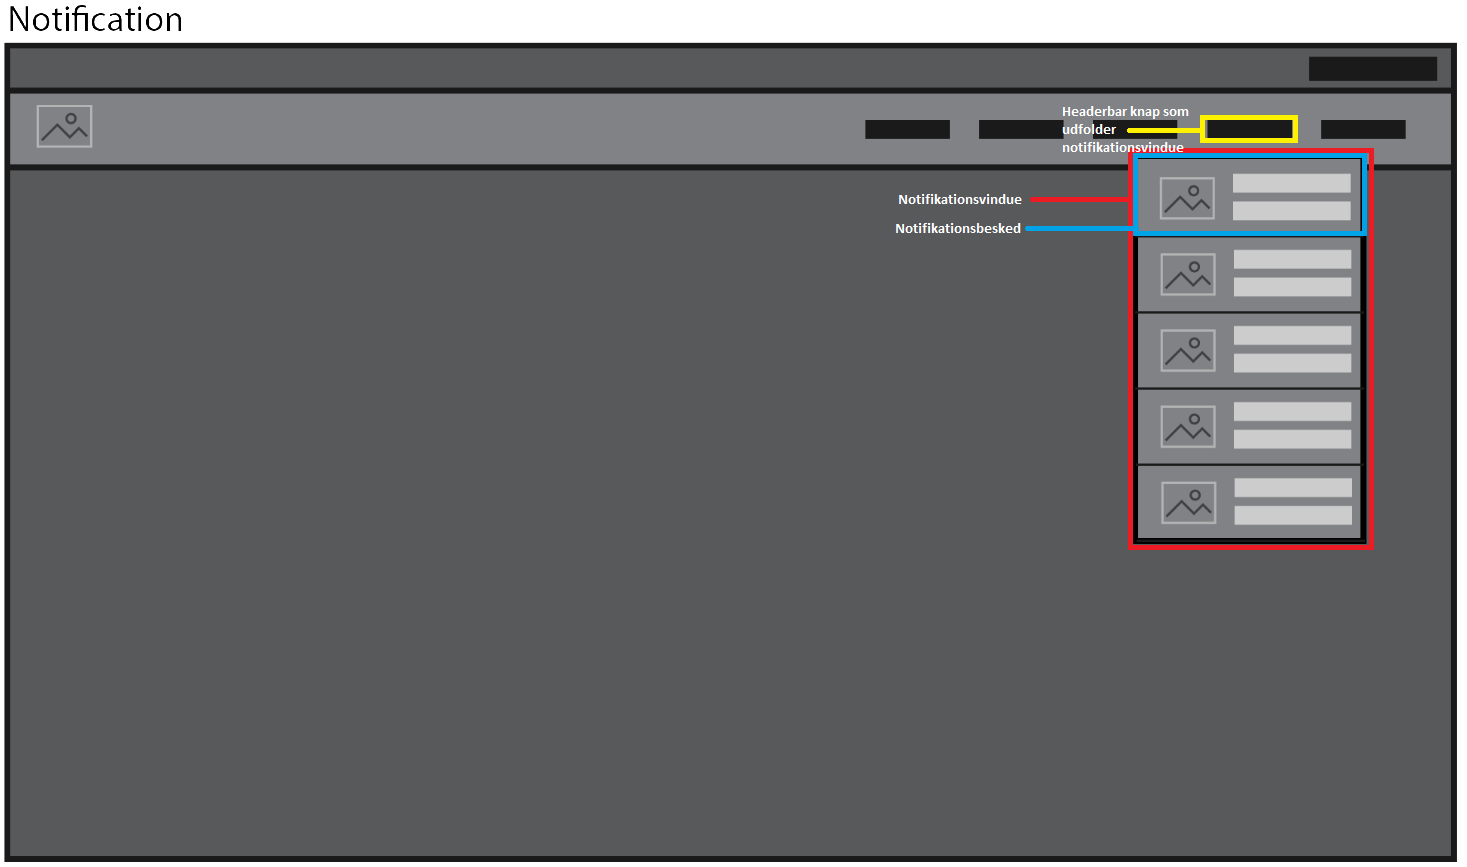
\includegraphics[width=\textwidth]{SoftwareDesign/MVVMDesigns/Graphics/noti_wirefame.png}
    \caption{Frame for Notifikations vinduet}
    \label{fig:wire_noti}
\end{figure}

\subsection{Besked opbygning}
Notifikationsvinduet skal kunne indeholde forskellige typer beskeder, og det skal være let at tilføje nye beskeder. Hvis beskederne indeholder en besked på over 15 karakter, bliver de resterende karakter ikke vist i vinduet. Beskederne hentes fra databasen, hvor deres given typer definerer, hvordan de vises i notifikationsvinduet. I de følgende delafsnit forklares hvordan dette designes og figur \ref{fig:cd_noti} viser et klassediagram af operationen.

\begin{figure}[H]
    \centering
    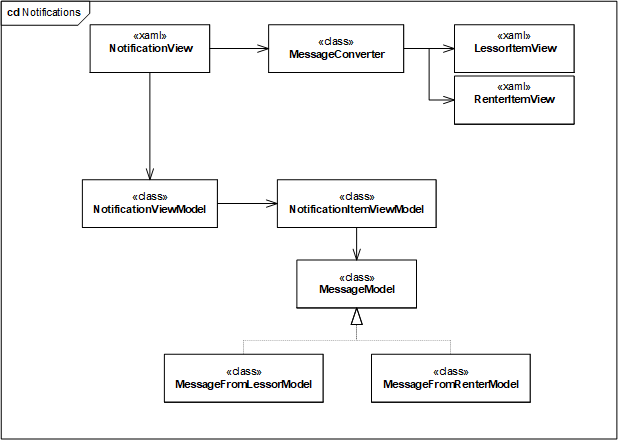
\includegraphics[width=\textwidth]{SoftwareDesign/MVVMDesigns/Graphics/cd_notification.png}
    \caption{Klassediagram for notifikationer}
    \label{fig:cd_noti}
\end{figure}

\subsection{MessageConverter}
En bruger vil modtage notifikationer, når han interagere med applikationen, fx når der enten lejes eller udlejes en bil. Disse notifikationer 'pop'er up' og vises i headerbaren. Hver type besked vises forskelligt, der skal således runtime differenceres mellem besked typerne. Hertil bruges en 'valueconverter', som konverterer en besked til et 'wpf item' i notifikationsvinduet - en notifikationsbesked, repræsenteret som en blok inde i notifikationsvinduet (Se figur \ref{fig:wire_noti}. Hvert besked har dets egen model, og for at illustrere informationer, skal der laves et tilhørende 'ItemView' for beskedmodellen - 'LessorItemView' er det visuelle vindue for informationen gemt i beskeden 'MessageFromLessorModel'. 
Hvis systemet udvides og der tilføjes flere typer beskeder, kan de let tilføjes ved at oprette et nyt ItemView, samt at beskederne nedarver fra MessageModel. 

\subsection{Interaktion med modeller og database}
For hvert gang der registreres nye beskeder for den specifikke bruger fra databasen, opdateres notifikationsvinduet. Når notifikationsvinduet aktiveres, vil det altid vise alle ulæste beskeder - når brugeren trykker på en notifikationsbesked, navigeres han til et andet vindue, som viser hele beskedens indhold, notifikationsbeskeden fjernes herefter fra notifikationsvinduet. Der loades de 10 nyeste beskeder fra databasen af gangen - brugeren har mulighed for at hente flere. 

\section{Design af MessageView}
I forlængelse med Notifikationsvinduet, skal brugeren have mulighed for at navigere til hvert besked, således han/hun kan læse alt indholdet for beskeden. Når der bliver trykket på en notfikationsbesked, så navigerer systemet til MessageView'et. Vinduet skal bestå af to sektioner: 
\begin{enumerate}
    \item Den venstre side af vinduet skal vise alle brugerens beskeder
    \item Den højre side skal vise indholdet af den besked, som brugeren har valgt.  
    \begin{itemize}
        \item Udlejer respons: Her vises beskeden fra udlejeren, samt om han har godkent bilanmodningen. Hvis dette er tilfældet, angives lejerens email og et link til bilprofilen
        \item Lejer anmodning: Her vises beskeden fra lejer - udlejeren kan godkende eller afvise anmodningen i notifkationsvinduet. 
    \end{itemize}
\end{enumerate}
Nedenfor ses 'framet' for vinduet. Her ses hvordan de to sektioner er opdelt: \\
\begin{figure}[H]
    \centering
    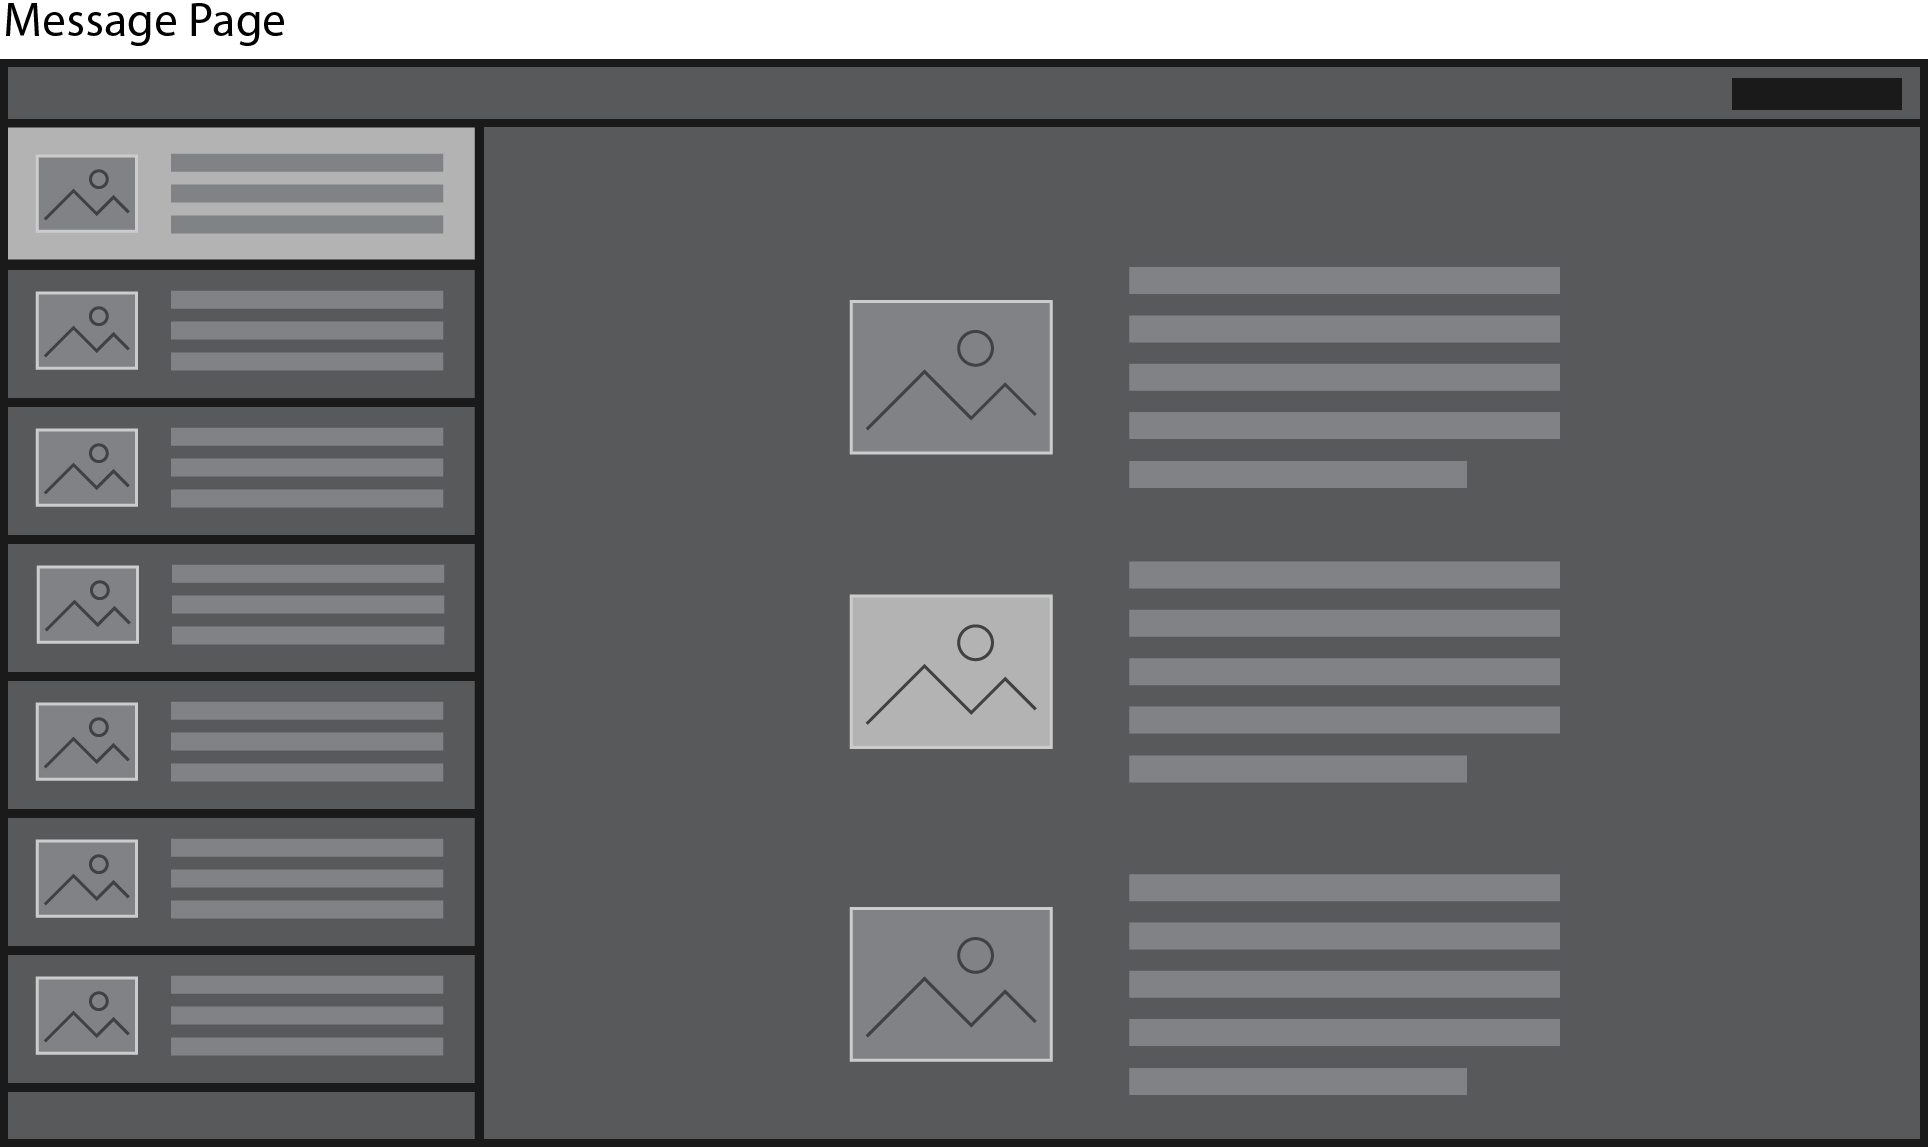
\includegraphics[width=\textwidth]{SoftwareDesign/MVVMDesigns/Graphics/MessageView.png}
    \caption{Frame for MessageView}
    \label{fig:wire_message}
\end{figure}

\subsection{Interaktion med modeller og database}
Brugerens beskeder vil være et 1:1 forhold med notifikationsvinduet, her skal der vises de samme beskeder - beskederne er dog ikke statiske i den forstand, at de loades igen, når der skiftes mellem Notifikationsvinduet og Messagevinduet. Der vil være en søgebar til rådighed, hvor brugeren kan indtaste navnet på en bruger han/hun har kommunikeret med. Her returnerer databasen alle beskeder med den bruger, ellers angives at der ikke blev fundet nogen. 
\end{document}